\chapter{PENGUJIAN DAN ANALISIS}
\label{chap:pengujiananalisis}

% Ubah bagian-bagian berikut dengan isi dari pengujian dan analisis

Pada bab ini dipaparkan hasil pengujian serta analisa dari desain sistem dan implementasi. Pengujian dilakukan guna mengetahui tingkat kesalahan dan menarik kesimpulan dari sistem yang telah dibuat.

Pada proses oengujian digunakan salah satu layanan \textit{Google} yaitu \textit{Google Colaboratory} dengan spesifikasi \textit{hardware} seperti pada Tabel \ref{tab:spek-colab}. Sedangkan untuk spesifikasi \textit{hardware} komputer penulis dapat dilihat pada Tabel \ref{tab:spek-pc}.
\begin{table}[h!]
	\begin{center}
		\begin{tabular}{ |c|c| } 
			\hline
			\textbf{Procesor} & Intel Xeon Processor @ 2.3 GHz\\
			\hline 
			\textbf{Graphic Card} & Tesla K80 12 GB GDDR5 VRAM\\
			\hline 
			\textbf{RAM} & 16 GB\\ 
			\hline
		\end{tabular}
		\caption{Spesifikasi \textit{hardware Google Colaboratory}}
		\label{tab:spek-colab}
	\end{center}
\end{table} 

\begin{table}[h!]
	\begin{center}
		\begin{tabular}{ |c|c| } 
			\hline
			\textbf{Procesor} & Intel(R) Core(TM) i5-10400F CPU @ 2.90GHz\\
			\hline 
			\textbf{Graphic Card} & Nvidia GeForce GTX 1650 4 GB GDDR6\\
			\hline 
			\textbf{RAM} & 8 GB\\ 
			\hline
		\end{tabular}
		\caption{Spesifikasi \textit{hardware} Komputer yang Digunakan}
		\label{tab:spek-pc}
	\end{center}
\end{table}

Pengujian dilakukan dengan membagi menjadi beberapa bagian yaitu sebagai berikut

\begin{enumerate}
	\item Pengujian jenis \textit{backbone}
	\item Pengujian jenis teknik validasi
\end{enumerate}

\section{Pengujian Jenis \textit{Backbone}}
\label{sec:pengujian-backbone}

\subsection{Resnet 50}
\label{resnet50}

Resnet-50 merupakan salah satu \textit{Image Classification} dari CNN dengan jumlah layer sebanyak 50. Gambar \ref{fig:resnet50-arch} adalah arsitektur dari Resnet50.

\begin{figure}[ht]
	\centering
	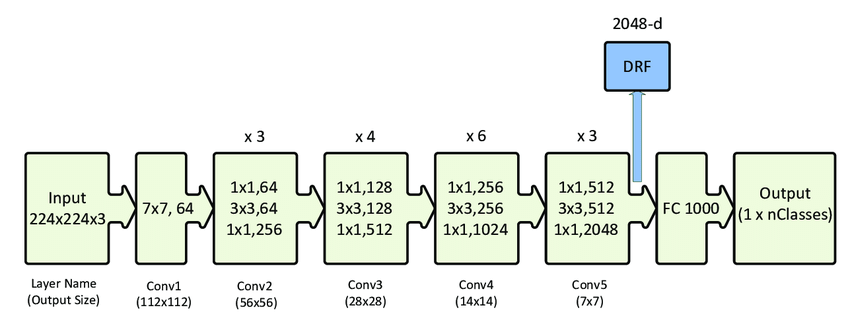
\includegraphics[scale=0.3]{gambar/resnet50.png}
	\caption{Gambaran Arsitekture ResNet50}
	\label{fig:resnet50-arch}
\end{figure} 

Gambar \ref{fig:resnet50-hasil} merupakan hasil deteksi yang dilakukan menggunakan \textit{backbone} resnet-50.
\begin{figure}[ht]
	\centering
	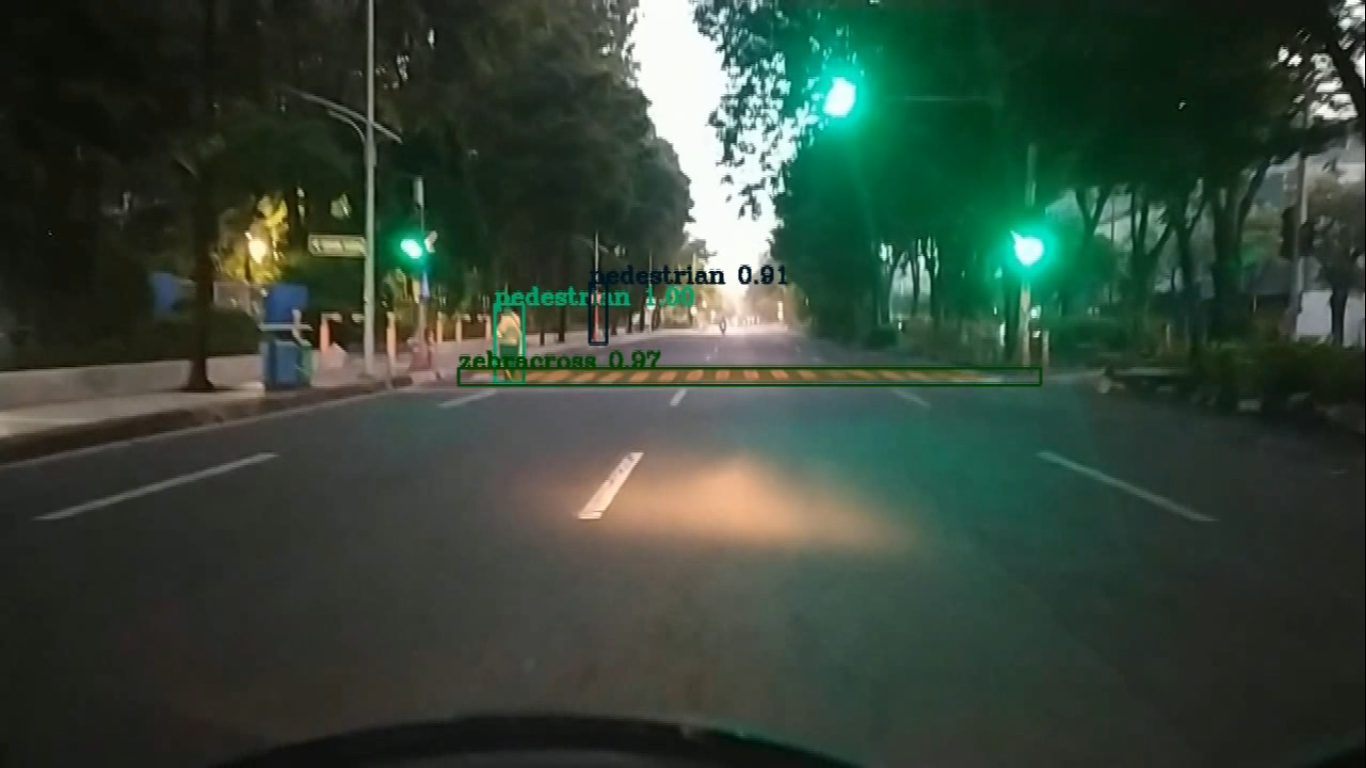
\includegraphics[scale=0.15]{gambar/hasil-resnet50.png}
	\caption{Gambaran Hasil Deteksi ResNet50}
	\label{fig:resnet50-hasil}
\end{figure} 




\subsection{Resnet 101}
\label{resnet101}

Resnet-101 merupakan salah satu \textit{Image Classification} dari CNN dengan jumlah layer sebanyak 101. Gambar \ref{fig:resnet101-arch} adalah arsitektur dari Resnet-101.

\begin{figure}[ht]
	\centering
	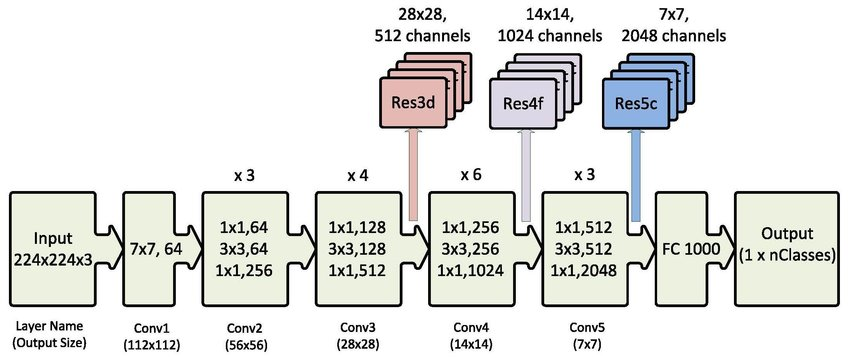
\includegraphics[scale=0.3]{gambar/resnet101.png}
	\caption{Gambaran Arsitekture ResNet101}
	\label{fig:resnet101-arch}
\end{figure} 

Gambar \ref{fig:resnet101-hasil} merupakan hasil deteksi yang dilakukan menggunakan \textit{backbone} resnet-101.
\begin{figure}[ht]
	\centering
	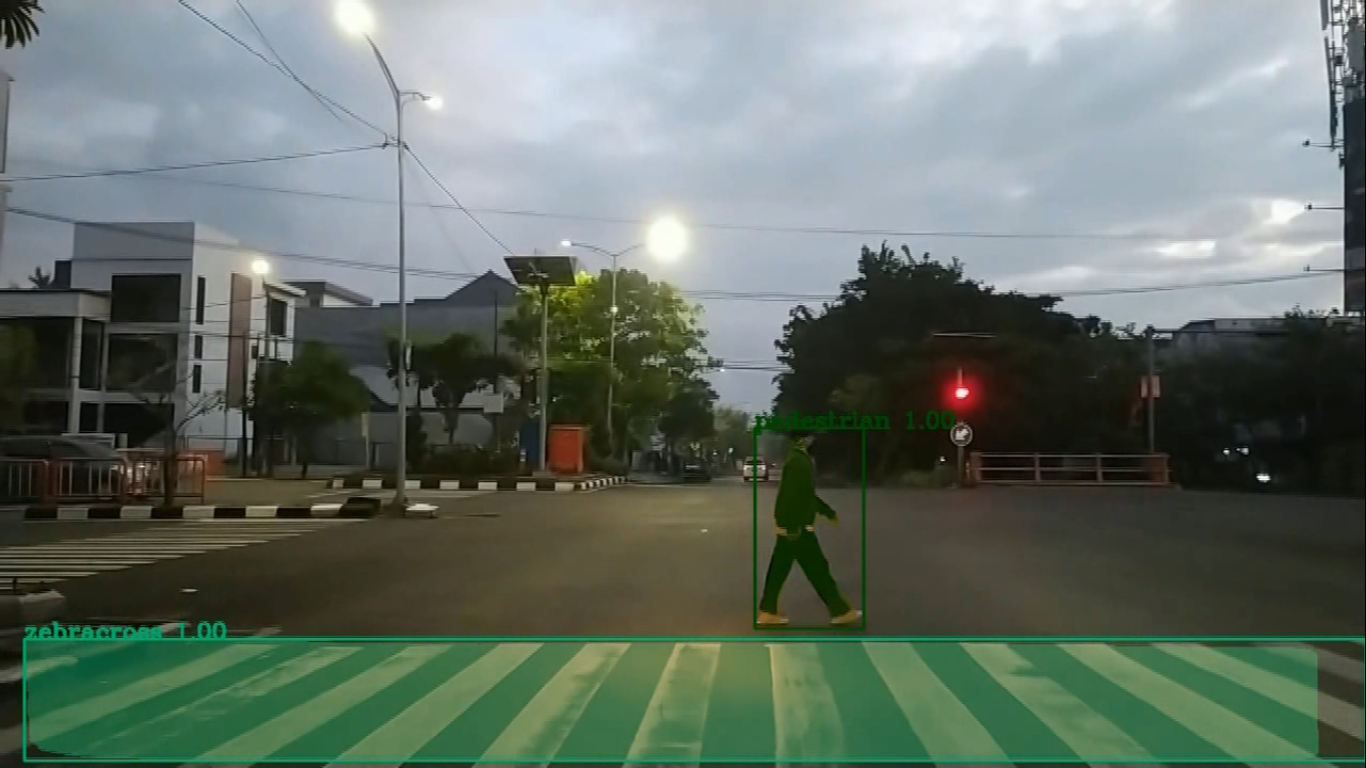
\includegraphics[scale=0.15]{gambar/hasil-resnet101.png}
	\caption{Gambaran Hasil Deteksi ResNet101}
	\label{fig:resnet101-hasil}
\end{figure} 


\subsection{MobileNet V1}
\label{mobilenetv1}

\subsection{MobileNet V2}
\label{mobilenetv2}

\section{Pengujian Jenis Teknik Validasi}
\label{sec:pengujian-validation}

\subsection{Pengujian dengan Pemisahan Data Validasi}
\label{normal-validasi}

\subsection{Pengujian dengan \textit{K Fold Cross Validation}}
\label{cross-validasi}